\section{Base Case} \label{baseCase}

\subsection{In The Early Stages}
The Living Lab had two websites: the main website that is used as the front-facing which contains some information about the Living Lab as shown in Figure \ref{mainWebsiteIMG}, and a private website that is used to compile some of the information of working with the Living Lab as shown in Figure \ref{privateWebsiteIMG}. At the start of the Living Lab project, the main website served its purpose on having a digital platform that is accessible to the public. As the project goes on, some of the information is held on a Google Drive, and some of the information are compiled in the private website.

\begin{figure}
\begin{center}
  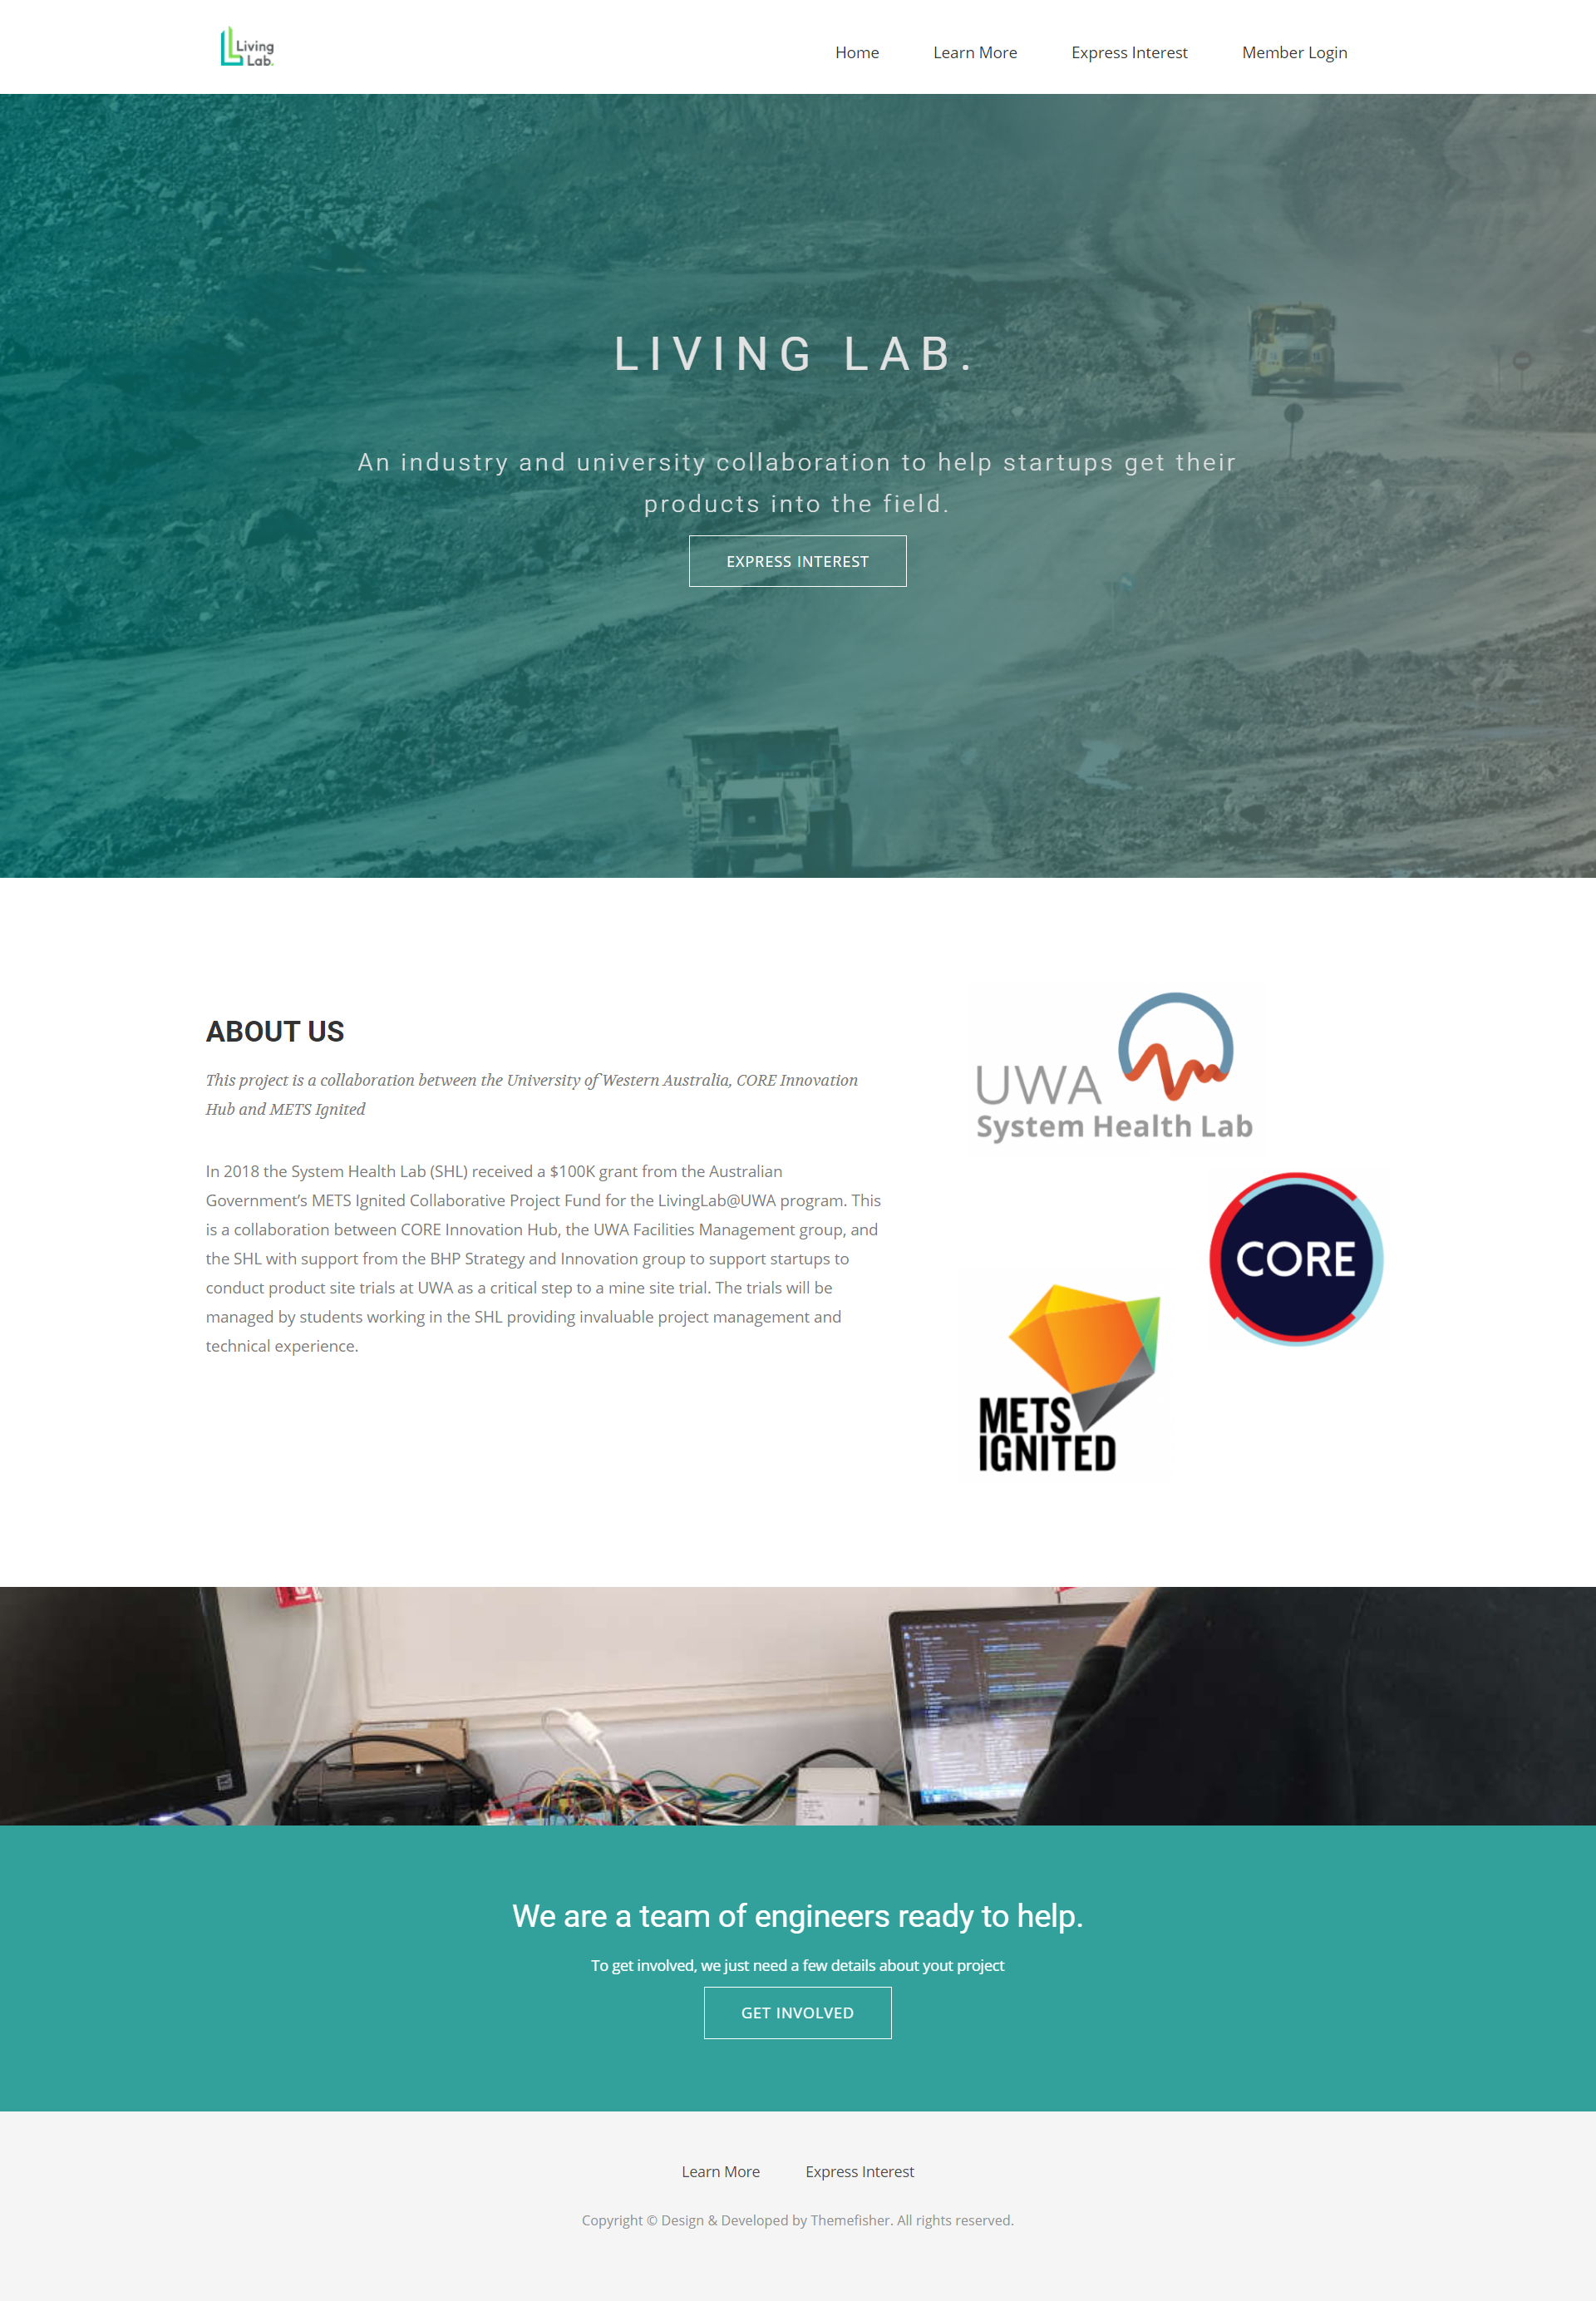
\includegraphics[width=\textwidth]{BaseCase/main-website-1.png} \\
  \caption{The Main Website Before July 2020} \label{mainWebsiteIMG}
\end{center}
\end{figure}

\begin{figure}
\begin{center}
  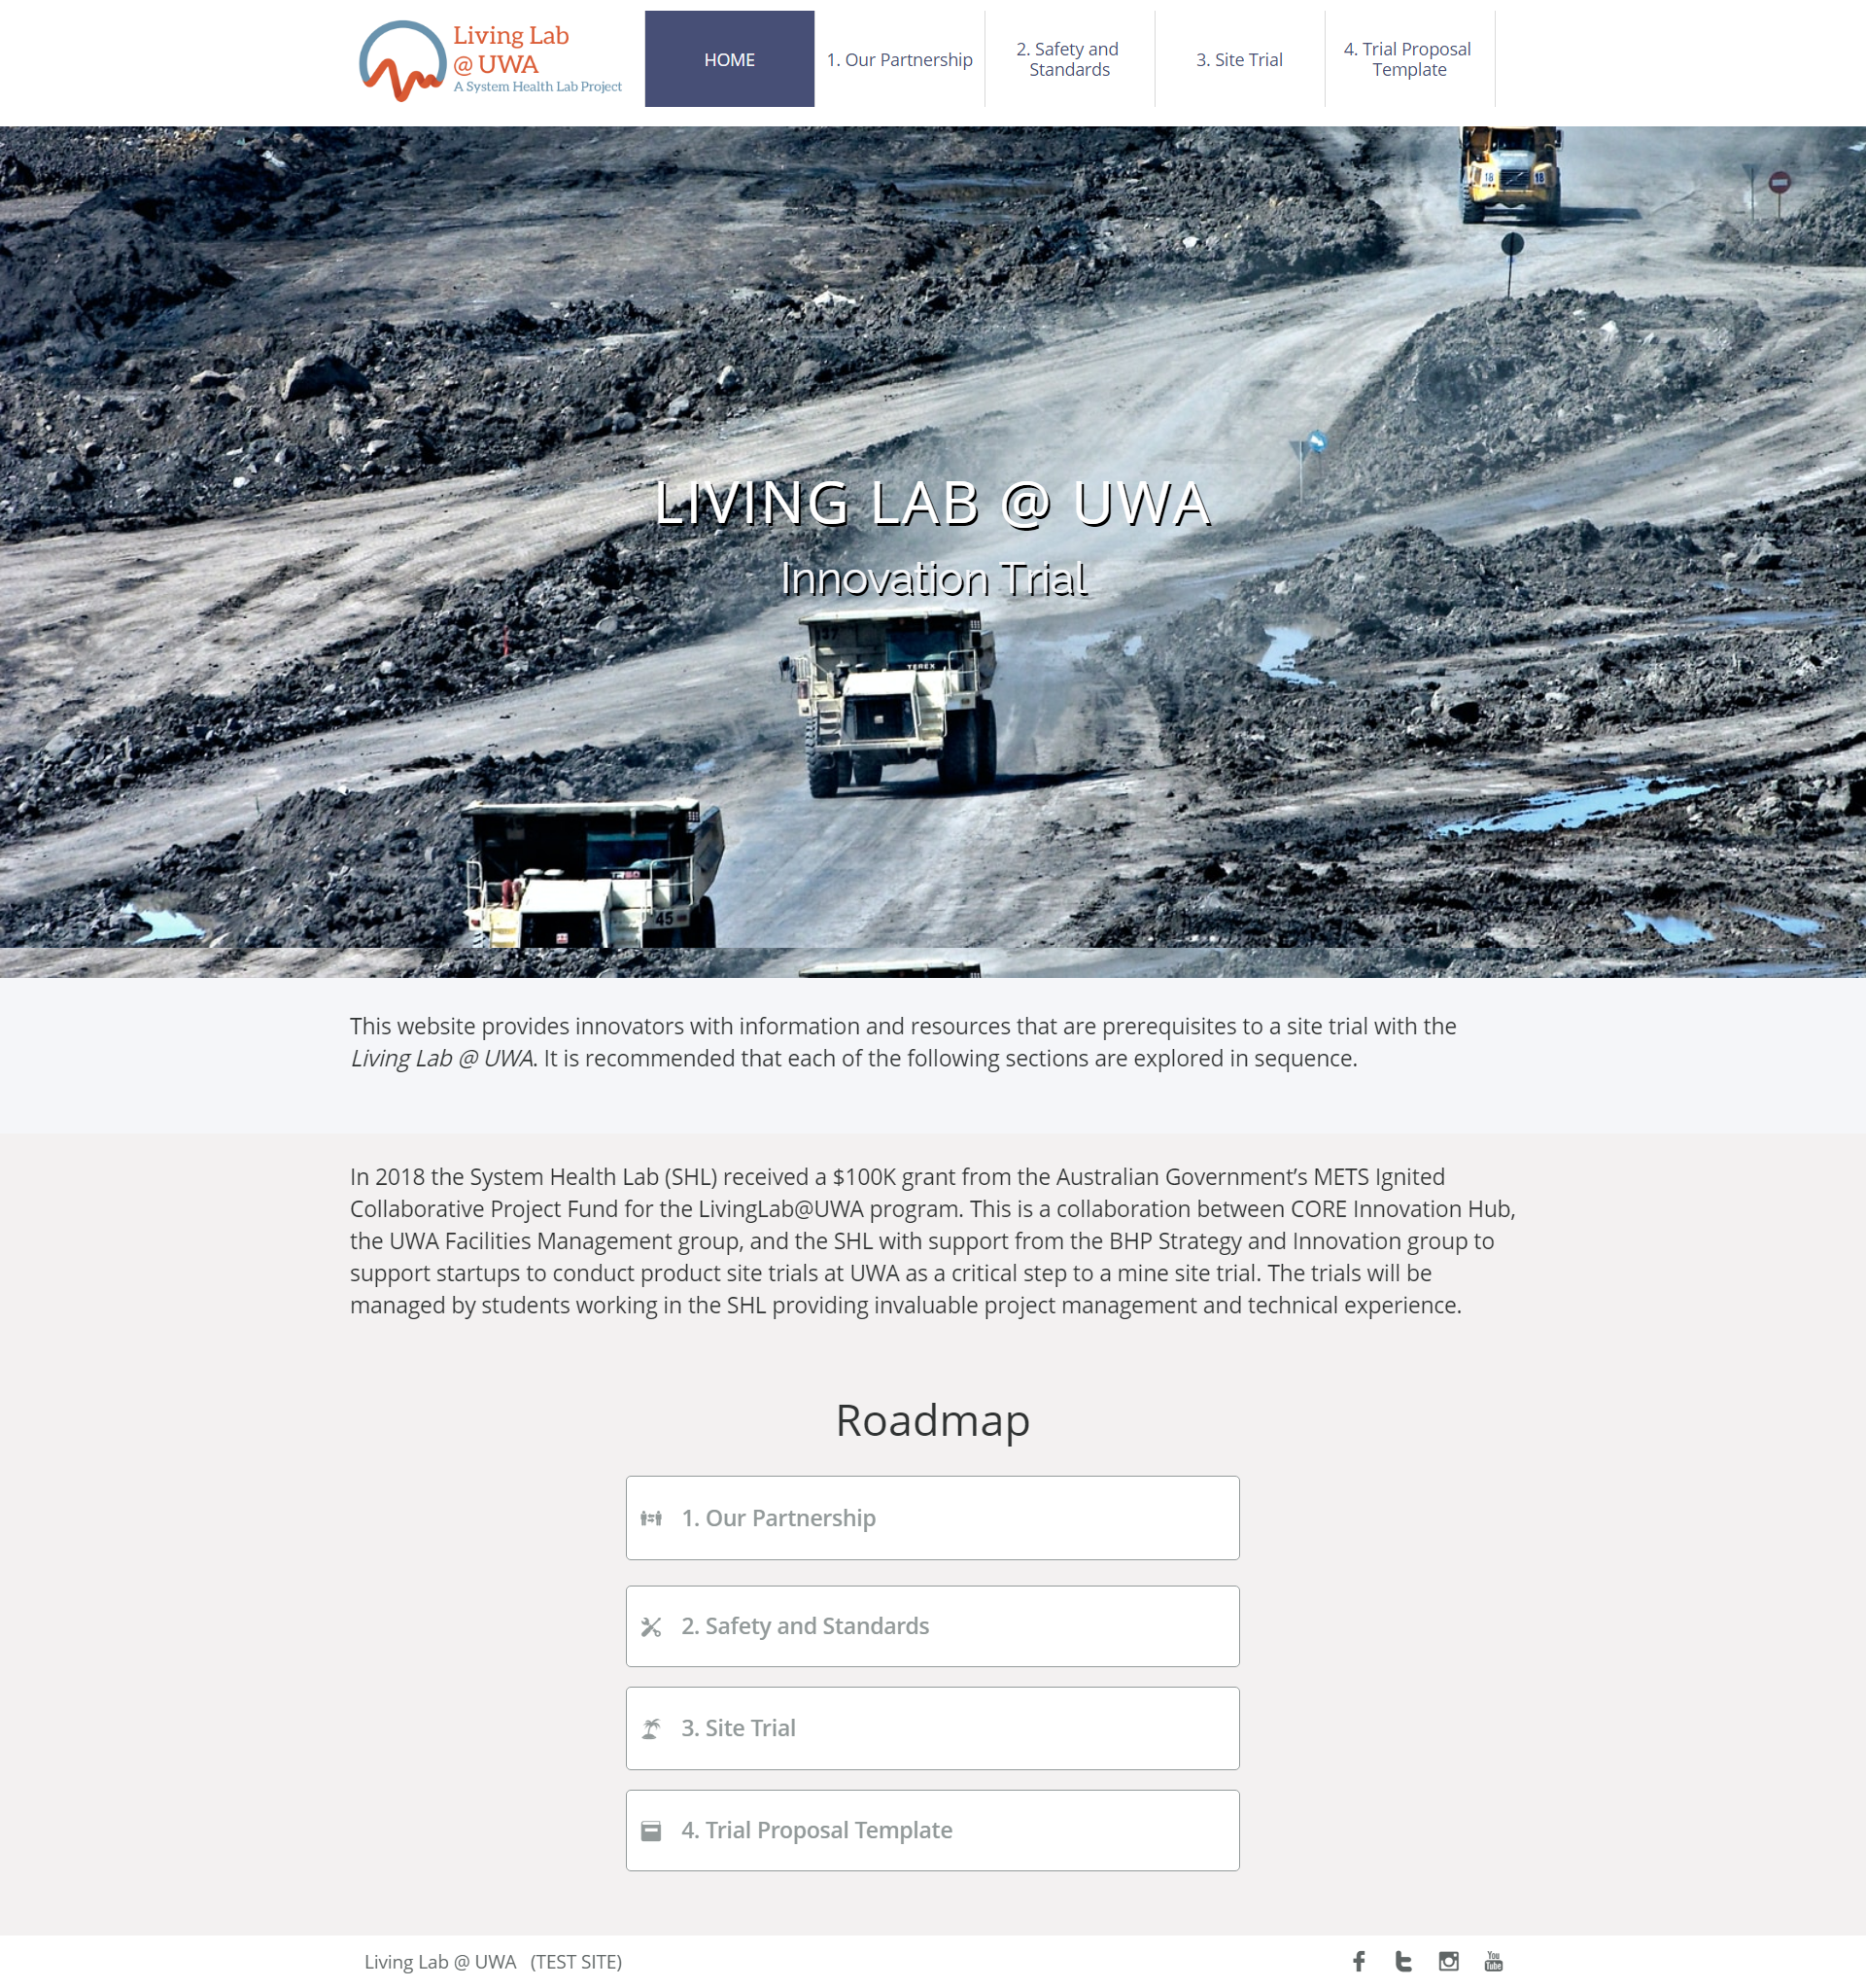
\includegraphics[width=\textwidth]{BaseCase/private-website.png} \\
  \caption{The Private Website To Compile Information} \label{privateWebsiteIMG}
\end{center}
\end{figure}

\subsection{Issue}
The current state of the web platforms presented issues compiled in Table \ref{issues}.

\begin{table}[htp]

\begin{center}
\begin{tabular}{  p{5cm} | p{6cm} | p{6cm} }
\textbf{Issue} & \textbf{Impact} & \textbf{The Solution} \\
\hline

%  Private Website
 The private website has information, but not shown in public &  Marketing opportunity lost & Move the information of the private website to the main website\\ \hline

%  Google Drive Information
 Some of the information of about the capability of the Living Lab is hidden in Google Drive  & Marketing opportunity lost. Time loss in needing to find basic information in Google Drive. &  Incorporate the appropriate information with the main website \\ \hline

% Roadmap Navigation
 The roadmap is shown in the navigation bar. &  The graphical representation of the roadmap is not engaging, and takes too much spaces in terms of the main navigation. & Use a graphical representation of a roadmap to indicate step, and move the roadmap over to a page of roadmap \\ \hline

% Web Technology
 The main website used Hugo - web technology for creating basic websites which is great for static content. &  Hugo is limited in its feature in reusing components which makes updating code harder. Furthermore, the development team is not familiar of the tool. & Use a modern web framework that is known by the development team, and fully-featured for the purpose of UI development.\\ \hline

\end{tabular} \label{issues.}
\end{center}
\caption{Issues In The Early Stages} \label{issues}
\end{table}
